\section{The experimental effort}\label{sec:experiments}

During the last decade the field of \bbonu\ searches has exploded. Three experiments (EXO-200 \cite{Albert:2014awa, Auger:2012ar}, KamLAND-Zen \cite{Asakura:2014lma, Gando:2012zm} and GERDA-I \cite{Agostini:2013mzu}) have released physics results, excluding  lifetimes below $10^{25}$~years for the \bbonu\ of \XE\ (EXO-200 and KamLAND-Zen) and the \bbonu\ mode of \GE\ (GERDA-I). 
Five more experiments will start operations in the next few years.  {\scshape Majorana} \cite{Abgrall:2013rze}(germanium diodes), NEXT-100 \cite{Gomez-Cadenas:2014dxa} (a high-pressure gas xenon TPC), CUORE  \cite{Giachero:2014hva} (TeO$_{2}$ crystal bolometers), SNO+ \cite{Biller:2014eha} (Tellurium  dissolved in liquid scintillator) and the SuperNEMO demonstrator \cite{Guzowski:2014ina} (using Selenium). We refer to all these as the
``current generation'' of \bbonu\ searches. The typical exposures deployed will be of the order of 20 kg $\cdot$yr for the SuperNEMO demonstrator, 50--100 kg $\cdot$yr for germanium experiments (GERDA and  {\scshape Majorana} ), 300 kg $\cdot$yr for the xenon TPCs (EXO-200 and NEXT-100), and around 500 kg $\cdot$yr for CUORE, SNO+ and KamLAND-ZEN. The expected background in the ROI (measured in the case of 
EXO-200, KamLAND-Zen and GERDA-I, computed by Monte Carlo calculations for all the others) varies between $\sim$10 and $\sim$ 100 events per ton and year. The expected sensitivity to the Majorana neutrino mass (\mbb), after some 3 years run, of several of these experiments is in the range of 100 meV \cite{Gomez-Cadenas:2015twa}.

The performance of the various experiments can be summarized in terms of their basic operational parameters. These are: a) the \bb\ source isotope; b) the energy resolution $\Delta E$ (usually expressed as FWHM); the specific background rate ($c$) in the region of interest (ROI) around \Qbb (normally expressed in \ckky); the signal detection efficiency, $\varepsilon$; and the source mass M. The exposure is obtained multiplying the source mass by the running time. 

%The basic operational parameters of the experiments of the current generation are listed in Table~\ref{tab:ParamsCurrentGeneration}. The size of the uncertainties associated to the parameters varies according to the state of development of each project.  The smallest uncertainties correspond to the running experiments, which have \emph{measured} their operational parameters. CUORE and GERDA-II have assessed their expected performance with setups operating under conditions similar to those of the final experiment. The remaining experiments base their expectations on results obtained with R\&D prototypes, ancillary measurements and Monte Carlo simulations. 
%
%%%%%%%%%%%
%\begin{table}[!]
%\centering
%\caption{Basic operational parameters of the \bbonu-decay experiments of the current generation: \bb\ source isotope, energy resolution (FWHM), $\Delta E$; background rate in the region of interest around \Qbb; signal detection efficiency, $\varepsilon$; and source mass.} \label{tab:ParamsCurrentGeneration}
%\small
%\begin{tabular*}{\textwidth}{@{\extracolsep{\fill}} l c D{.}{.}{3.0} D{.}{.}{0.5} c D{.}{.}{3.0}}
%\toprule
%Experiment & Isotope & \multicolumn{1}{c}{$\Delta E$} & \multicolumn{1}{c}{Bkgnd.\ rate} & \multicolumn{1}{c}{$\varepsilon$} & \multicolumn{1}{c}{Mass} \\
%           &         & \multicolumn{1}{c}{(keV)} & \multicolumn{1}{c}{(keV$^{-1}$~kg$^{-1}$~yr$^{-1}$)} & \multicolumn{1}{c}{$(\%)$} & \multicolumn{1}{c}{(kg)} \\ \midrule
%%
%CUORE-0\hair\textsuperscript{\itshape a} \cite{Giachero:2014hva} & \TE\ & 5 & 0.23 & 78 & 11 \\
%%
%CUORE\hair\textsuperscript{\itshape b} \cite{Alessandria:2011rc} & \TE\ & 5 & 0.04 & 87 & 206 \\
%%
%GERDA-I\hair\textsuperscript{\itshape a} \cite{Agostini:2013mzu} & \GE\ &   5 & 0.013 & 62 & 15 \\
%%
%GERDA-II\hair\textsuperscript{\itshape b} \cite{Macolino:2014vya} & \GE\ & 3 & 0.001 & 66 & 33 \\
%%
%EXO-200\hair\textsuperscript{\itshape a} \cite{Albert:2014awa} & \XE\ & 88 & 0.002 & 85 & 76 \\
%%
%KamLAND-Zen\hair\textsuperscript{\itshape a} \cite{Gando:2012zm, Asakura:2014lma} & \XE\ & 243 & 0.00014  & 25 & 348 \\
%%
%{\scshape Majorana}\textsuperscript{\itshape c} \cite{Abgrall:2013rze} & \GE\ & 4 & 0.0009 & 70 & 25 \\
%%
%NEXT-100\hair\textsuperscript{\itshape c} \cite{Gomez-Cadenas:2014dxa} & \XE\ &  17 & 0.0005  & 30 & 91 \\
%%
%SNO+\hair\textsuperscript{\itshape c} \cite{Biller:2014eha} & \TE\ & 264 & 0.0001  & 15 & 800 \\
%%
%SuperNEMO-D\hair\textsuperscript{\itshape c} \cite{Guzowski:2014ina} & \SE\ & 120 & 0.0005 & 30 & 7 \\ 
%%%
%\bottomrule \\[-8pt]
%%
%\multicolumn{6}{l}{\textsuperscript{\itshape a} \footnotesize The experiment is running and has measured its operational parameters.} \\[-2pt]
%\multicolumn{6}{l}{\textsuperscript{\itshape b} \footnotesize The experiment has proven its feasibility with a demonstrator.} \\[-2pt]
%\multicolumn{6}{l}{\textsuperscript{\itshape c} \footnotesize The operational parameters are estimations based on R\&D results and simulations. } \\
%\end{tabular*}
%\end{table}
%%%%%%%%%%%

The total background in the ROI per year $b$ is readily obtained as $b = c \cdot M \cdot t \cdot \Delta E$. The sensitivity to the Majorana neutrino mass of a background free experiment improves with the square root of the exposure. Contrarily, in the limit of background--limited experiments, the sensitivity of \bbonu\ experiments can be approximated by (see discussion in \cite{Gomez-Cadenas:2015twa}):

\begin{equation}
{S}(\mbb) = \propto \sqrt{1/\varepsilon}\ \left(\frac{c~\Delta E}{M~t}\right)^{1/4}\,. \label{eq:Sensitivity3}
\end{equation}
%%%

Since the background limits dramatically the sensitivity of a double beta decay experiment, any extrapolation of scale requires a huge effort. For example, the NEXT-100 experiment foresees to reach a sensitivity of 
$\mbb < 100$~meV for an exposure of 300 kg $\cdot$ year and a background rate of $\sim$1 count per 100 kg and year in the ROI. For an exposure of 1 ton $\cdot$ year, NEXT-100 would register about 10 background counts per year in the ROI and its sensitivity would be in the background-dominated regime. To explore the inverse hierarchy it is necessary to reach $\mbb < 20$~meV. Upgrading the NEXT detector by simply building a detector or larger mass (without adding an improvement to the technology that would drastically reduce the background) would not work, since in the background-dominated regime, an improvement of a factor 5 in $\mbb$ requires an improvement of 625 in the product $b/E$. Thus, if $b$~ does not improve, the total exposure would approach some 200 tons $\cdot$ year. Unfortunately, even assuming a very long running period, say of 10 years, building a 20 ton high pressure xenon chamber appears difficult. 

On the other hand, the HPXe technology should permit to reach a resolution of at least 0.5 \% FWHM at \Qbb\ \cite{Alvarez:2012kua}, thus reducing the ROI to some 12 keV. Even more important, as we will show in this paper, adding a magnetic field to NEXT could reduce the specific background in the ROI to about $5 \times 10^{-5}$~ \ckky. Then, $b \sim 0.6$ counts per year and ton and the upgraded experiment would be in the background-free regime. Therefore to improve the sensitivity to $\mbb$~by a factor 5, one needs to reduce $b/E$~by ``only'', a factor 25, which in turn translates in a ``moderate'' exposure of some 2 ton $\cdot$ year. 


%%%%%%%%%%
\begin{figure}
\centering
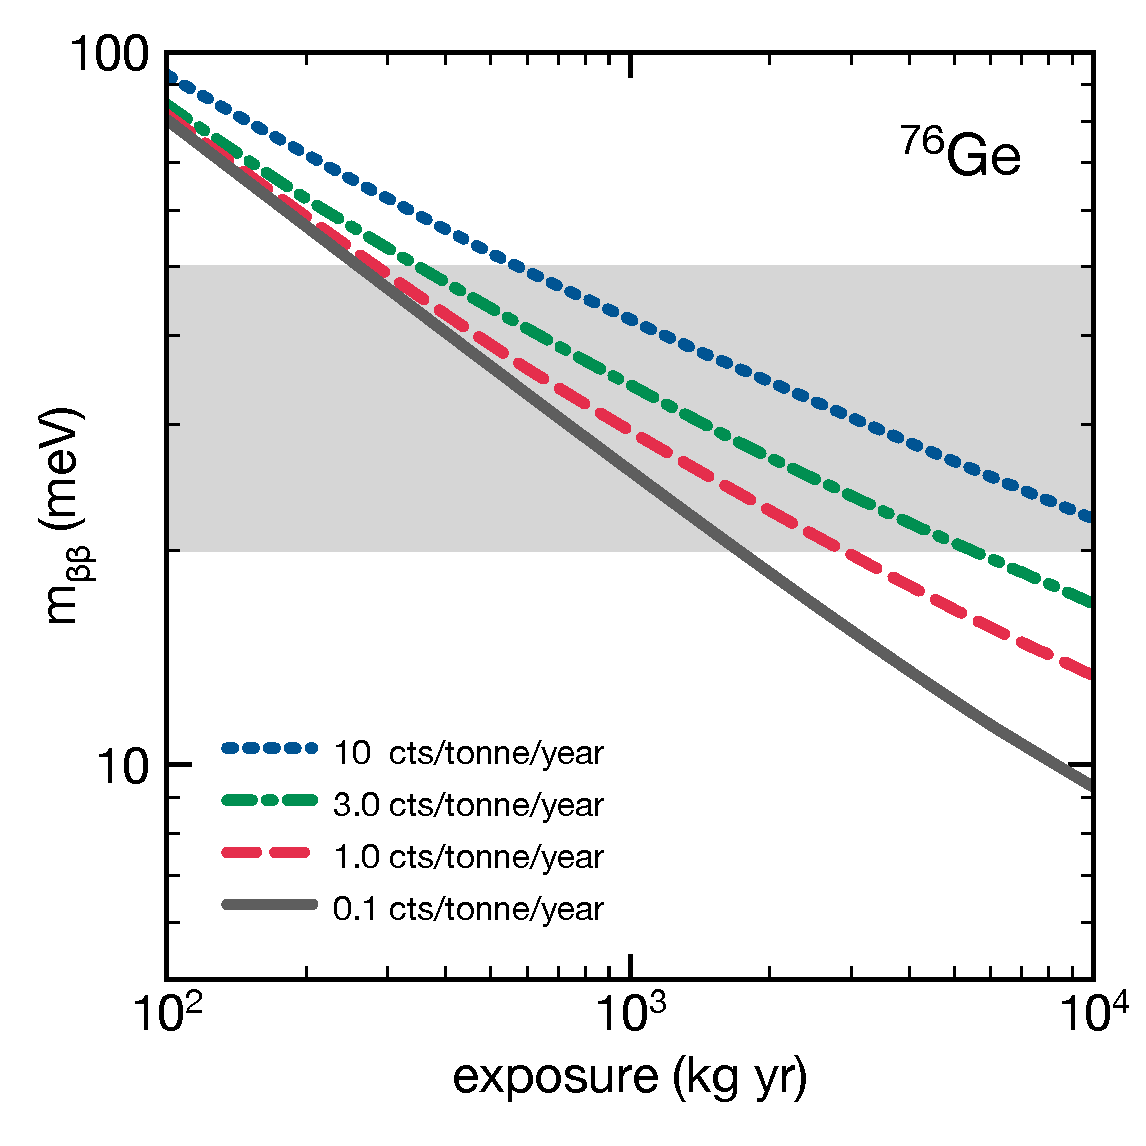
\includegraphics[width=0.45\textwidth]{img/FutureGe76.pdf}
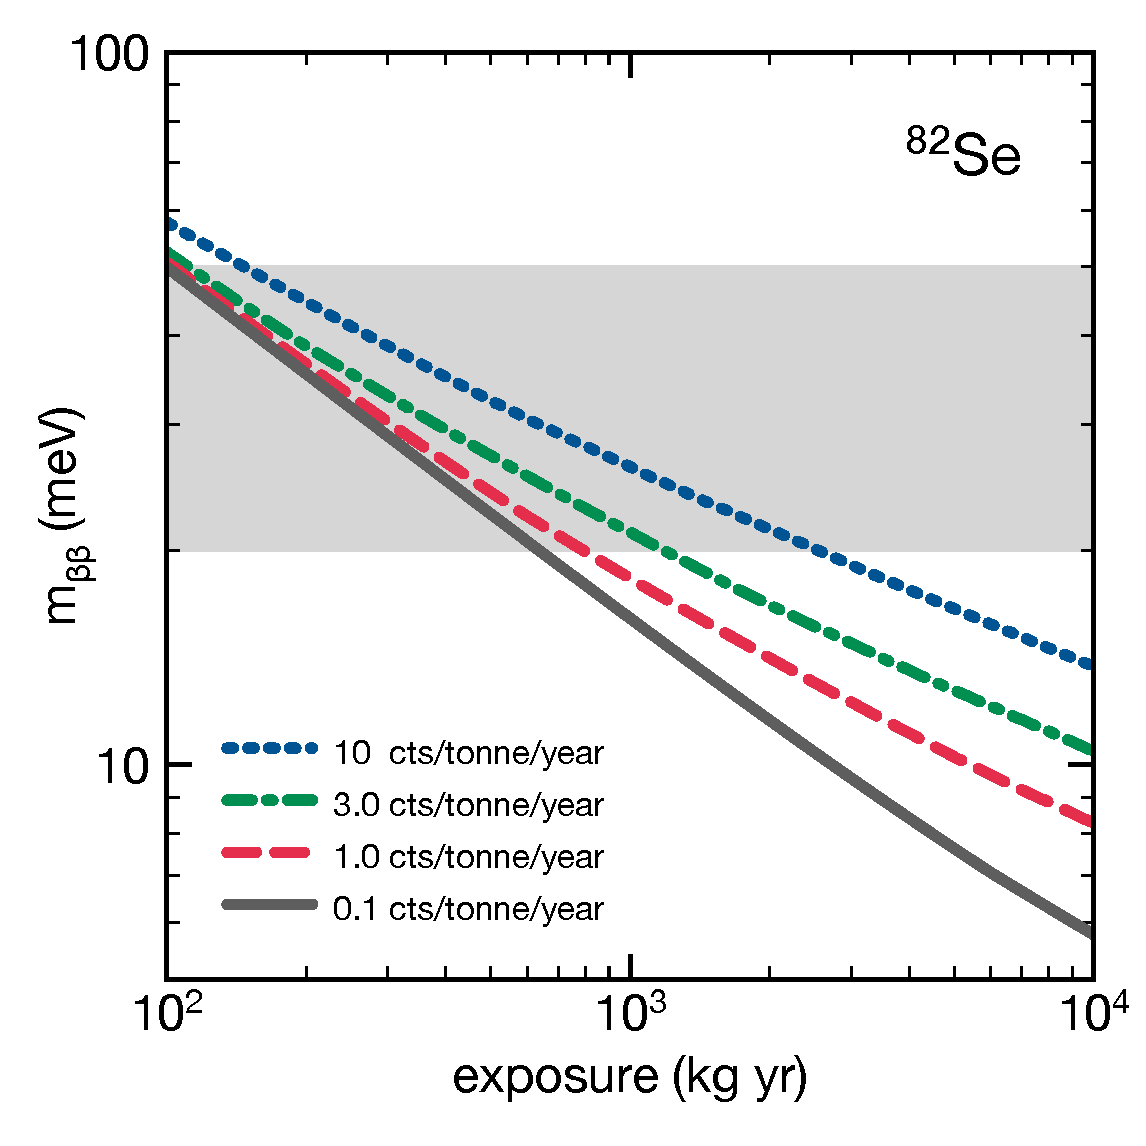
\includegraphics[width=0.45\textwidth]{img/FutureSe82.pdf}
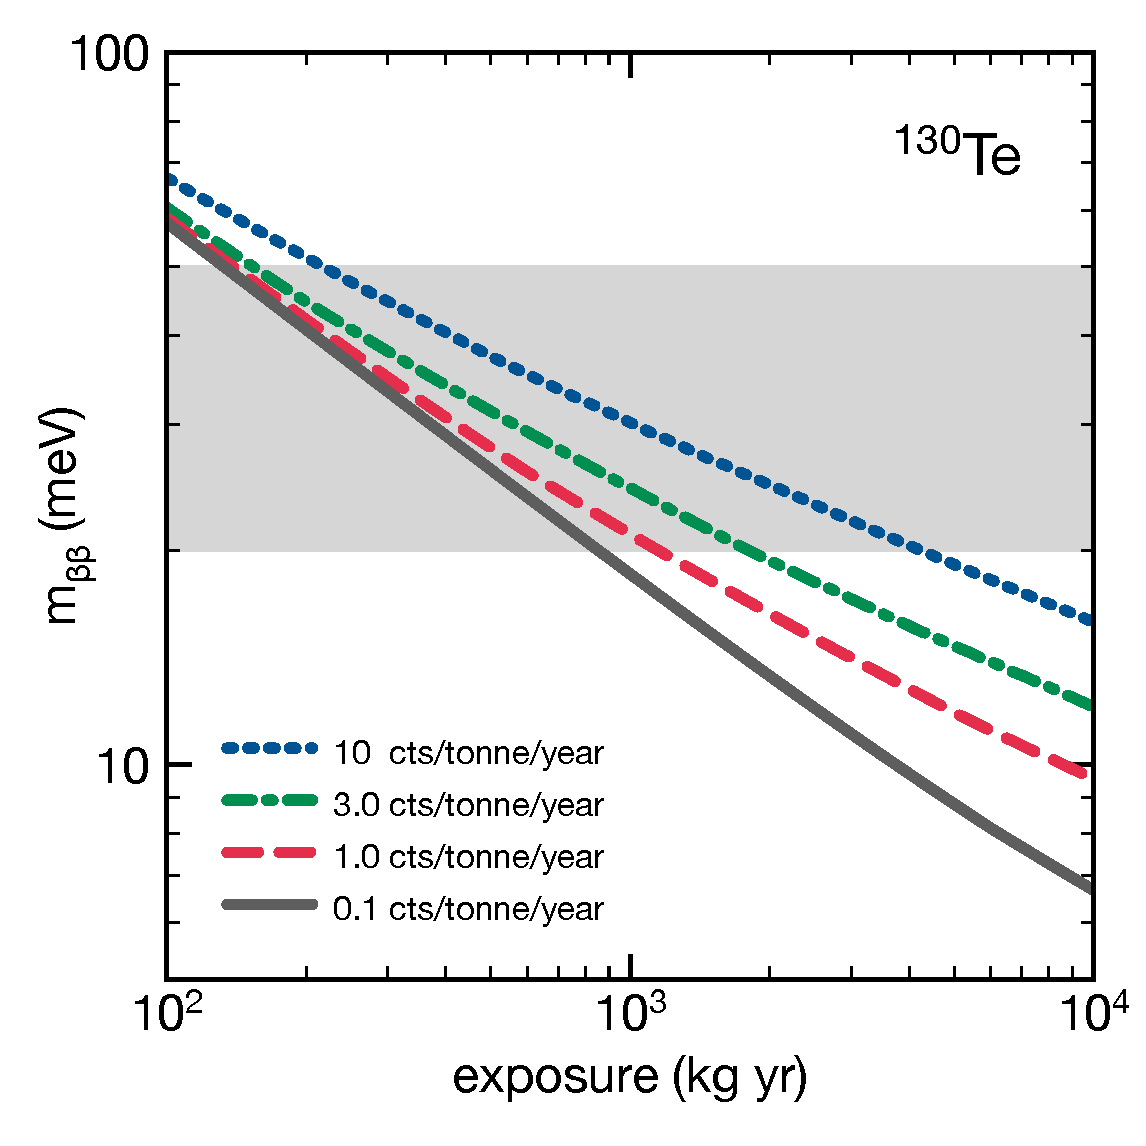
\includegraphics[width=0.45\textwidth]{img/FutureTe130.pdf}
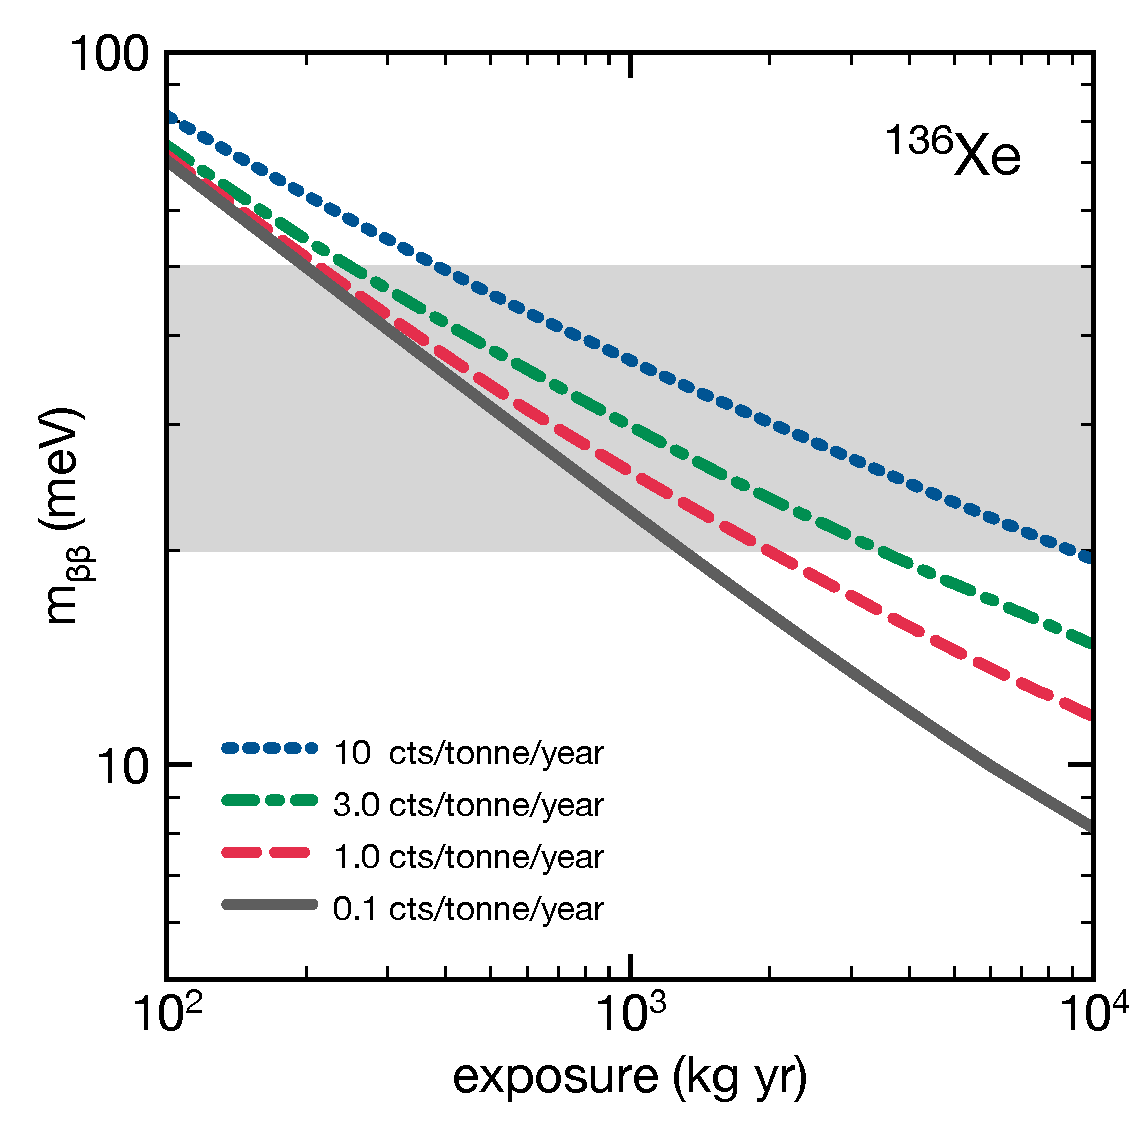
\includegraphics[width=0.45\textwidth]{img/FutureXe136.pdf}
\caption{Exposure dependence of the \mbb\ sensitivity (at 90\% CL) of perfectly-efficient experiments based on 4 different isotopes and with 4 different assumptions for the background rate in the ROI. The grey band represents the inverted-hierarchy region of neutrino masses.} \label{fig:FutureGen}
\end{figure}
%%%%%%%%%%

Figure \ref{fig:FutureGen} quantifies the above discussion, showing the exposure dependence of the \mbb\ sensitivity (at 90\% CL) of perfectly-efficient experiments based on 4 different isotopes and with 4 different assumptions for the background rate in the ROI. Notice that the grey band represents the inverted-hierarchy region of neutrino masses. If perfectly efficient, the putative NEXT upgraded detector that we have just described, with a background rate of 0.6 counts per ton and year would cover the inverted hierarchy with an exposure of less than 2 ton $\cdot$~year. Including a realistic efficiency (in the range of 30\%), would push the required exposure to some 6 ton $\cdot$ year, reachable with a detector deploying a fiducial mass of around one ton of isotope.  

